\label{LastPage}
\section{Wichtige Formeln}

$\sin^2(b)+\cos^2(b)=1 \qquad \tan(b)=\frac{\sin(b)}{\cos(b)}$
  
  
\subsection{Funktionswerte für Winkelargumente}
  \renewcommand{\arraystretch}{1.5}
  \begin{minipage}{5cm}
    \begin{tabular}[c]{ |c|c||c|c|c| }
        \hline
      deg & rad & sin & cos & tan\\
      \hline
      0\symbol{23} & 0 & 0 & 1 & 0\\
      \hline
      30\symbol{23} & $\frac{\pi}{6}$ & $\frac{1}{2}$ & $\frac{\sqrt{3}}{2}$ &
      $\frac{\sqrt{3}}{3}$\\
      \hline
      45\symbol{23} & $\frac{\pi}{4}$ & $\frac{\sqrt{2}}{2}$ & $\frac{\sqrt{2}}{2}$
      & 1\\
      \hline
      60\symbol{23} & $\frac{\pi}{3}$ & $\frac{\sqrt{3}}{2}$ & $\frac{1}{2}$ &
      $\sqrt{3}$\\
      \hline      
    \end{tabular}     
  \end{minipage}
  \begin{minipage}{4.3cm}
    \begin{tabular}[c]{ |c|c||c|c|}
        \hline
      deg & rad & sin & cos\\
      \hline
      90\symbol{23} & $\frac{\pi}{2}$ & 1 & 0\\
      \hline  
      120\symbol{23} & $\frac{2\pi}{3}$ & $\frac{\sqrt{3}}{2}$ & $-\frac{1}{2}$ \\
      \hline
      135\symbol{23} & $\frac{3\pi}{4}$ & $\frac{\sqrt{2}}{2}$ & $-\frac{\sqrt{2}}{2}$\\
      \hline
      150\symbol{23} & $\frac{5\pi}{6}$ & $\frac{1}{2}$ & $-\frac{\sqrt{3}}{2}$\\
      \hline
    \end{tabular}     
  \end{minipage}
  \begin{minipage}{4.5cm}
    \begin{tabular}[c]{ |c|c||c|c| }
        \hline
      deg & rad & sin & cos\\
      \hline
      180\symbol{23} & $\pi$ & 0 & -1\\
      \hline  
      210\symbol{23} & $\frac{7\pi}{6}$ & $-\frac{1}{2}$ & $-\frac{\sqrt{3}}{2}$\\
      \hline
      225\symbol{23} & $\frac{5\pi}{4}$ & $-\frac{\sqrt{2}}{2}$ & $-\frac{\sqrt{2}}{2}$\\
      \hline
      240\symbol{23} & $\frac{4\pi}{3}$ & $-\frac{\sqrt{3}}{2}$ & $-\frac{1}{2}$\\
      \hline
    \end{tabular}     
  \end{minipage}
  \begin{minipage}{4.5cm}
    \begin{tabular}[c]{ |c|c||c|c| }
        \hline
      deg & rad & sin & cos\\
      \hline
      270\symbol{23} & $\frac{3\pi}{2}$ & -1 & 0\\
      \hline  
      300\symbol{23} & $\frac{5\pi}{3}$ & $-\frac{\sqrt{3}}{2}$ & $\frac{1}{2}$\\
      \hline
      315\symbol{23} & $\frac{7\pi}{4}$ & $-\frac{\sqrt{2}}{2}$ & $\frac{\sqrt{2}}{2}$\\
      \hline
      330\symbol{23} & $\frac{11\pi}{6}$ & $-\frac{1}{2}$ & $\frac{\sqrt{3}}{2}$\\
      \hline
    \end{tabular}     
  \end{minipage}
  \renewcommand{\arraystretch}{1}
  
\subsection{Periodizität}
  $\cos(a+k\cdot2\pi)=\cos(a) \qquad \sin(a+k\cdot2\pi)=\sin(a) \qquad
  (k \in \mathbb{Z})$
  
\subsection{Quadrantenbeziehungen}
  \begin{tabbing}
      xxxxxxxxxxxxxxxxxxxxxxxxxxxxxxxxxx \= \kill
      $\sin(-a)=-\sin(a)$ \> $\cos(-a)=\cos(a)$\\
    $\sin(\pi - a)=\sin(a)$ \> $\cos(\pi - a)=-\cos(a)$\\
    $\sin(\pi + a)=-\sin(a)$ \> $\cos(\pi +a)=-\cos(a)$\\
    $\sin\left(\frac{\pi}{2}-a \right)=\sin\left(\frac{\pi}{2}+a \right)=\cos(a)$ \>
    $\cos\left(\frac{\pi}{2}-a \right)=-\cos\left(\frac{\pi}{2}+a \right)=\sin(a)$  
    \end{tabbing}


\begin{minipage}{10.5cm}
  \subsection{Additionstheoreme}
    $\sin(a \pm b)=\sin(a) \cdot \cos(b) \pm \cos(a) \cdot \sin(b)$\\
    $\cos(a \pm b)=\cos(a) \cdot \cos(b) \mp \sin(a) \cdot \sin(b)$\\ 
    $\tan(a \pm b)=\frac{\tan(a) \pm \tan(b)}{1 \mp \tan(a) \cdot \tan(b)}$
    
  \subsection{Doppel- und Halbwinkel} 
    $\sin(2a)=2\sin(a)\cos(a)$\\
    $\cos(2a)=\cos^2(a)-\sin^2(a)=2\cos^2(a)-1=1-2\sin^2(a)$\\
    $\cos^2 \left(\frac{a}{2}\right)=\frac{1+\cos(a)}{2} \qquad
    \sin^2 \left(\frac{a}{2}\right)=\frac{1-\cos(a)}{2}$
    
  \subsection{Produkte}
    $\sin(a)\sin(b)=\frac{1}{2}(\cos(a-b)-cos(a+b))$\\
    $\cos(a)\cos(b)=\frac{1}{2}(\cos(a-b)+cos(a+b))$\\
    $\sin(a)\cos(b)=\frac{1}{2}(\sin(a-b)+\sin(a+b))$
    
  \subsection{Summe und Differenz}
    $\sin(a)+\sin(b)=2 \cdot \sin \left(\frac{a+b}{2}\right) \cdot
    \cos\left(\frac{a-b}{2}\right)$\\
    $\sin(a)-\sin(b)=2 \cdot \sin \left(\frac{a-b}{2}\right) \cdot
    \cos\left(\frac{a+b}{2}\right)$\\
    $\cos(a)+\cos(b)=2 \cdot \cos \left(\frac{a+b}{2}\right) \cdot
    \cos\left(\frac{a-b}{2}\right)$\\
    $\cos(a)-\cos(b)=-2 \cdot \sin \left(\frac{a+b}{2}\right) \cdot
    \cos\left(\frac{a-b}{2}\right)$\\
    $\tan(a) \pm \tan(b)=\frac{\sin(a \pm b)}{\cos(a)\cos(b)}$  
    
  \subsection{Euler}
    \begin{tabular}{lllllll}
      $\sin{\alpha} = \frac{e^{j\alpha} - e^{-j\alpha}}{2j}$ &

      $\cos{\alpha} = \frac{e^{j\alpha} + e^{-j\alpha}}{2}$ &
      
      $\tan{\alpha} = \frac{\sin \alpha}{\cos \alpha}$ &
      
      $ \qquad \qquad $ &
      
      $\sinh{\alpha} = \frac{e^\alpha - e^{-\alpha}}{2} $ &
      
      $\cosh{\alpha} = \frac{e^\alpha + e^{-\alpha}}{2} $ &
      
      $\tanh{\alpha} = \frac{e^\alpha - e^{-\alpha}}{e^\alpha + e^{-\alpha}}$
    \end{tabular}    
\end{minipage}
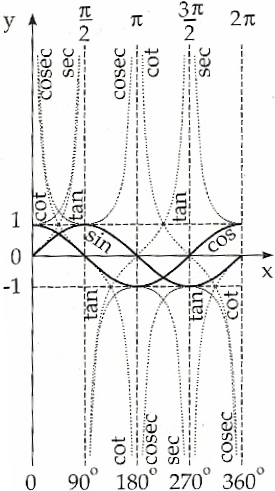
\includegraphics[width=0.2\textwidth]{bilder/funktionen_trigo}


  \subsection{Skalarprodukt und anderer Bullshit}
  \begin{tabular}{|p{3cm}|p{7cm}|p{7cm}|}
    \hline
    & Reelle Fourierreihe & Komplexe Fourierreihe \\
    \hline
    Skalarprodukt &  $\langle f;g \rangle = \frac{2}{T}\int\limits_0^Tf(t)\cdot
    g(t)\cdot dt $ & $\langle f;g \rangle = \frac{1}{T}\int\limits_0^Tf(t)\cdot
    \overline{g(t)}\cdot dt $ \\
    & $(I)\ \langle f;f \rangle > 0\ f"ur\ f\neq 0$ &
    $(I)\ \langle f;f \rangle > 0\ f"ur\ f\neq 0$ \\
    & $(II)\ \langle f;g \rangle = \langle g;f \rangle $ &
    $(II)\ \langle f;g \rangle = \overline{\langle g;f \rangle} $ \\
    & $(III) \langle r\cdot f;g\rangle = r\cdot\langle f;g\rangle,\ r\epsilon
    \mathbb R$ & $(III) \langle r\cdot f;g\rangle = r\cdot\langle f;g\rangle,\ 
    r\epsilon \mathbb R$
    \\
    \hline
    Länge (Norm): & \multicolumn{2}{|l|}{
    $\parallel f \parallel = \sqrt{\langle
    f;f \rangle} \Rightarrow y=3x^2+4 \rightarrow \sqrt{3\cdot3+4\cdot4}=5$ 
    } \\
    & \multicolumn{2}{|l|}{ $ (I)\ \parallel f \parallel > 0 f"ur f \neq 0$} \\
    & \multicolumn{2}{|l|}{ $ (II)\ \parallel f+g \parallel \leq \parallel f
    \parallel + \parallel g \parallel (Dreiecksgleichung)$} \\
    & \multicolumn{2}{|l|}{ $ (III)\ \parallel r\cdot f \parallel = |r| \cdot
    \parallel f \parallel , \ r \epsilon \mathbb R bzw. \parallel c\cdot
    f\parallel = |c|\cdot \parallel f \parallel, c\epsilon\mathbb C$} \\
    \hline
    Abstand: & \multicolumn{2}{|l|}{ $ \parallel f-g \parallel =
    |\sqrt{\langle f-g;f-g \rangle}| \Rightarrow
    |p-q|=(3x^2+4)-(x^2+7)=2x^2+11 \rightarrow
    \sqrt{2\cdot2+11\cdot11}=5\cdot\sqrt{5}$}
    \\
    \hline
    Winkel, Orthogonalit"at &
    \multicolumn{2}{|l|}{
    $\sphericalangle(f;g)=\arccos\left( \frac{\langle f;g \rangle}{\parallel f
    \parallel \cdot \parallel g \parallel} \right) = \arccos\left(\frac{\langle f;g 
    \rangle}{\sqrt{\langle f;f\rangle \cdot \langle g;g\rangle}}\right)$} \\
     & \multicolumn{2}{|l|}{$f \perp g\Leftrightarrow \langle f;g \rangle = 0$}
     \\
    
    
    \hline
    
  \end{tabular}


\section{Diverses}\label{Diverses}
\begin{tabbing}
  xxxxxxxxxxxxxxxxxxxxxxxxxxxx \= xxxxxxxxxxxxxxxxxxxxxxxxxxxxxx \= \kill
  $f'(z) = \lim \limits_{\Delta z \rightarrow 0} \frac{f(z + \Delta z) -
  f(z)}{\Delta z}$ \> $(a + b)^n = \sum_{k=0}^{n} \binom n k a^{n-k} \cdot b^k$ \>
  $(a \pm b)^3 =a^3 \pm  3 a^{2} b + 3 a b^2 \pm b^3 $\\ \\
  $x_{1,2} = \frac{-b \pm \sqrt{b^2 - 4ac}}{2a}$ \> $\binom n k = \frac{n!}{k!
  \cdot (n-k)!}$ \> $(a \pm b)^4 =a^4 \pm  4 a^{3} b + 6a^2b^2 \pm 4 a b^3 +
  b^4$\\ 
  \\Partielle Integration: $\int u(x) v'(x) dx = u(x)v(x) - \int u'(x) v(x) dx$
\end{tabbing}
